\documentclass[tikz, border=0pt]{standalone}
\usepackage{tikz}
\usetikzlibrary{arrows,automata,positioning}

\begin{document}
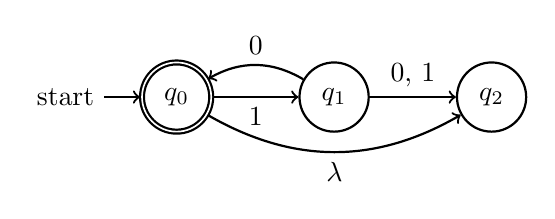
\begin{tikzpicture}[node distance=2cm, thick, auto]
% draw the states
\node[state, initial, accepting] (q_0) {\(q_0\)};
\node[state] (q_1) [right of=q_0] {\(q_1\)};
\node[state] (q_2) [right of=q_1] {\(q_2\)};
% draw the edges
\path[->] 
(q_0) edge node [swap] {1} (q_1)
edge [bend right] node [swap] {\(\lambda\)} (q_2)
(q_1) edge node {0, 1} (q_2)
(q_1) edge [bend right] [swap] node {0} (q_0)
;
\end{tikzpicture}
\end{document}